\newcommand{\atomr}{\textsf{r}}
\newcommand{\atomrp}{\textsf{r'}}
\newcommand{\atomg}{\textsf{g}}
\newcommand{\atomgp}{\textsf{g'}}

In this part we are going to briefly cover using propositional
formula to model systems. This is a common approach in hardware design
where a complete or partial model of a circuit or processor is defined in logic,
against which specifications of particular properties are checked.
The starting point is to work out a good way to represent/model a
system as a logical formula. In this part of the course, we will
consider systems modelled as simple state machines, with states and
transitions between the states describing how a system can
change/evolve. We will then convert this model into a propositional
formula.


To verify a system based on its model we then need a specification of
either good behaviour that we want to make sure follows from our model
or of bad behaviour which we want to ensure does not follow from the
model.  We formulate such a specification as a propositional formula
\emph{spec}, and then prove that the following is valid:
%
\begin{equation*}
\emph{model} \rightarrow \emph{spec}
\end{equation*}
%
The use of implication means that if the model holds then
the specification must hold. Alternatively, and equivalently,
we could state this as judgment $\emph{model} \vdash \emph{spec}$,
\ie{}, the specified behaviour follows from the model.

\section{State-transition models as propositions}

\paragraph{States}
Our running example will be a very simple traffic light comprising
a red light and a green light, with two possible states:
%
\setlength{\tabcolsep}{0.4em}
\begin{center}
  \begin{tabular}{m{1.1cm} m{1.5cm} m{1.1cm}}
    State 1 & & State 2 \\
{\scalebox{0.2}{
\includegraphics{images/red-on.pdf}}}
  &
  &
{\scalebox{0.2}{
\includegraphics{images/green-on.pdf}}}
\end{tabular}
\end{center}
%
Either the red light is on (left) or the green light is on (right),
but never both at the same time, and there is always at least one
light on. We will use two atoms (propositional
variables that can be true or false) $\atomr{}$ and $\atomg$ to represent the state of
each light separately, where:
%
\begin{itemize}
  \item \atomr{} means the red light is on; $\neg\atomr{}$ therefore
  means the red light is off;
  \item \atomg{} means the green light is on; $\neg\atomg{}$ means the
  green light is off.
\end{itemize}
%
The two valid states of the system can then be modelled as two propositions:
%
\begin{align*}
  \text{State 1} & \qquad\qquad \text{State 2} \\
  \atomr{} \wedge \neg\atomg{} &
  \qquad\qquad
  \neg\atomr{} \wedge \atomg{}
\end{align*}
%
For $n$-propositional atoms there are $2^n$ possible states that can
be modelled. Thus in our model, there are four possible states, two of
which we want to treat as valid (the above two).

\begin{exc}
Define a propositions for each of the two invalid states in the
traffic light.
\end{exc}

\noindent
\textbf{State transitions} \hspace{0.5em} So far we have modelled the states as propositions, but we also want to
model the behaviour of the system in terms of the possible
transitions between states. We can represent this
with a simple diagram:
%
\setlength{\tabcolsep}{0.4em}
\begin{center}
  \begin{tabular}{m{1.1cm} m{1.5cm} m{1.1cm}}
       State 1 & & State 2 \\[-0.5em]
{\scalebox{0.2}{
\includegraphics{images/red-on.pdf}}}
  &
    \xymatrix{
    \ar[rr]^{\textit{\normalsize{go}}} & & \\
     & & \ar[ll]^{\textit{\normalsize{stop}}}
    }
  &
{\scalebox{0.2}{
\includegraphics{images/green-on.pdf}}}
\end{tabular}
\end{center}
%
\ie{}, when just the red light is on it is possible to
transition to a state with just the green light on, and back again.

To model state transitions we will introduce two additional atoms
that model the future state of the lights in the system:
%
%
\begin{itemize}
\item \atomrp{} for the red light being on in the \emph{next time step};
\item \atomgp{} for the green light being on in the \emph{next time step}.
\end{itemize}
%
We can now express the above two transitions as implications:
%
\begin{align*}
  (\textit{go}) : \qquad & \atomr{} \wedge \neg\atomg{} \; \rightarrow \;
                           \neg\atomr{}' \wedge \atomg{}' \\
  (\textit{stop}): \qquad & \neg\atomr{} \wedge \atomg{} \; \rightarrow \;
                            \atomr{}' \wedge \neg\atomg{}'
\end{align*}
%
Said another way, (\textit{go}) defines that if State 1 is true now
we can move to State 2 in the future (in the ``next'' time step of the
system), and (\textit{stop}) conversely defines that if State 2 is
true now we can move to State 1 in the future.

We can now describe the full transition behaviour of the system as
the conjunction of the above two formula:
%
\begin{equation*}
\textit{model} =
(\atomr{} \wedge \neg\atomg{} \; \rightarrow \; \neg\atomr{}' \wedge
\atomg{}')
\, \wedge \,
(\neg\atomr{} \wedge \atomg{} \; \rightarrow \; \atomr{}' \wedge \neg\atomg{}')
\end{equation*}
%
This provides our model of the system. You might be wondering why we
don't add more to this, \eg{}, ruling out invalid states. We will come
back to this point in Section~\ref{subsec:whenisamodelgood}.

% TODO: guiding principles, why not and this with the valid states?
% want to make a small formula and this follows
% need to come back to this?

\paragraph{A general approach}

The general approach to modelling a system in this way is to:
%
\begin{itemize}
  \item Decide what to represent about the state space of the system
  and introduce propositional atoms for these components.
  \item Model future states using ``next step'' atoms (usually written with
  an apostrophe, and called the ``primed'' atoms, \eg{}, \atomrp{} is
  read as ``r prime'').
 \item Write a propositional formula \emph{model} using these
  variables which takes the conjunction of state transitions expressed
  as implications.
\end{itemize}

\begin{exc}
Write down a model for a more realistic traffic light, \ie{}, that can
be described by the following states and transitions:
%

\begin{center}
\scalebox{0.28}{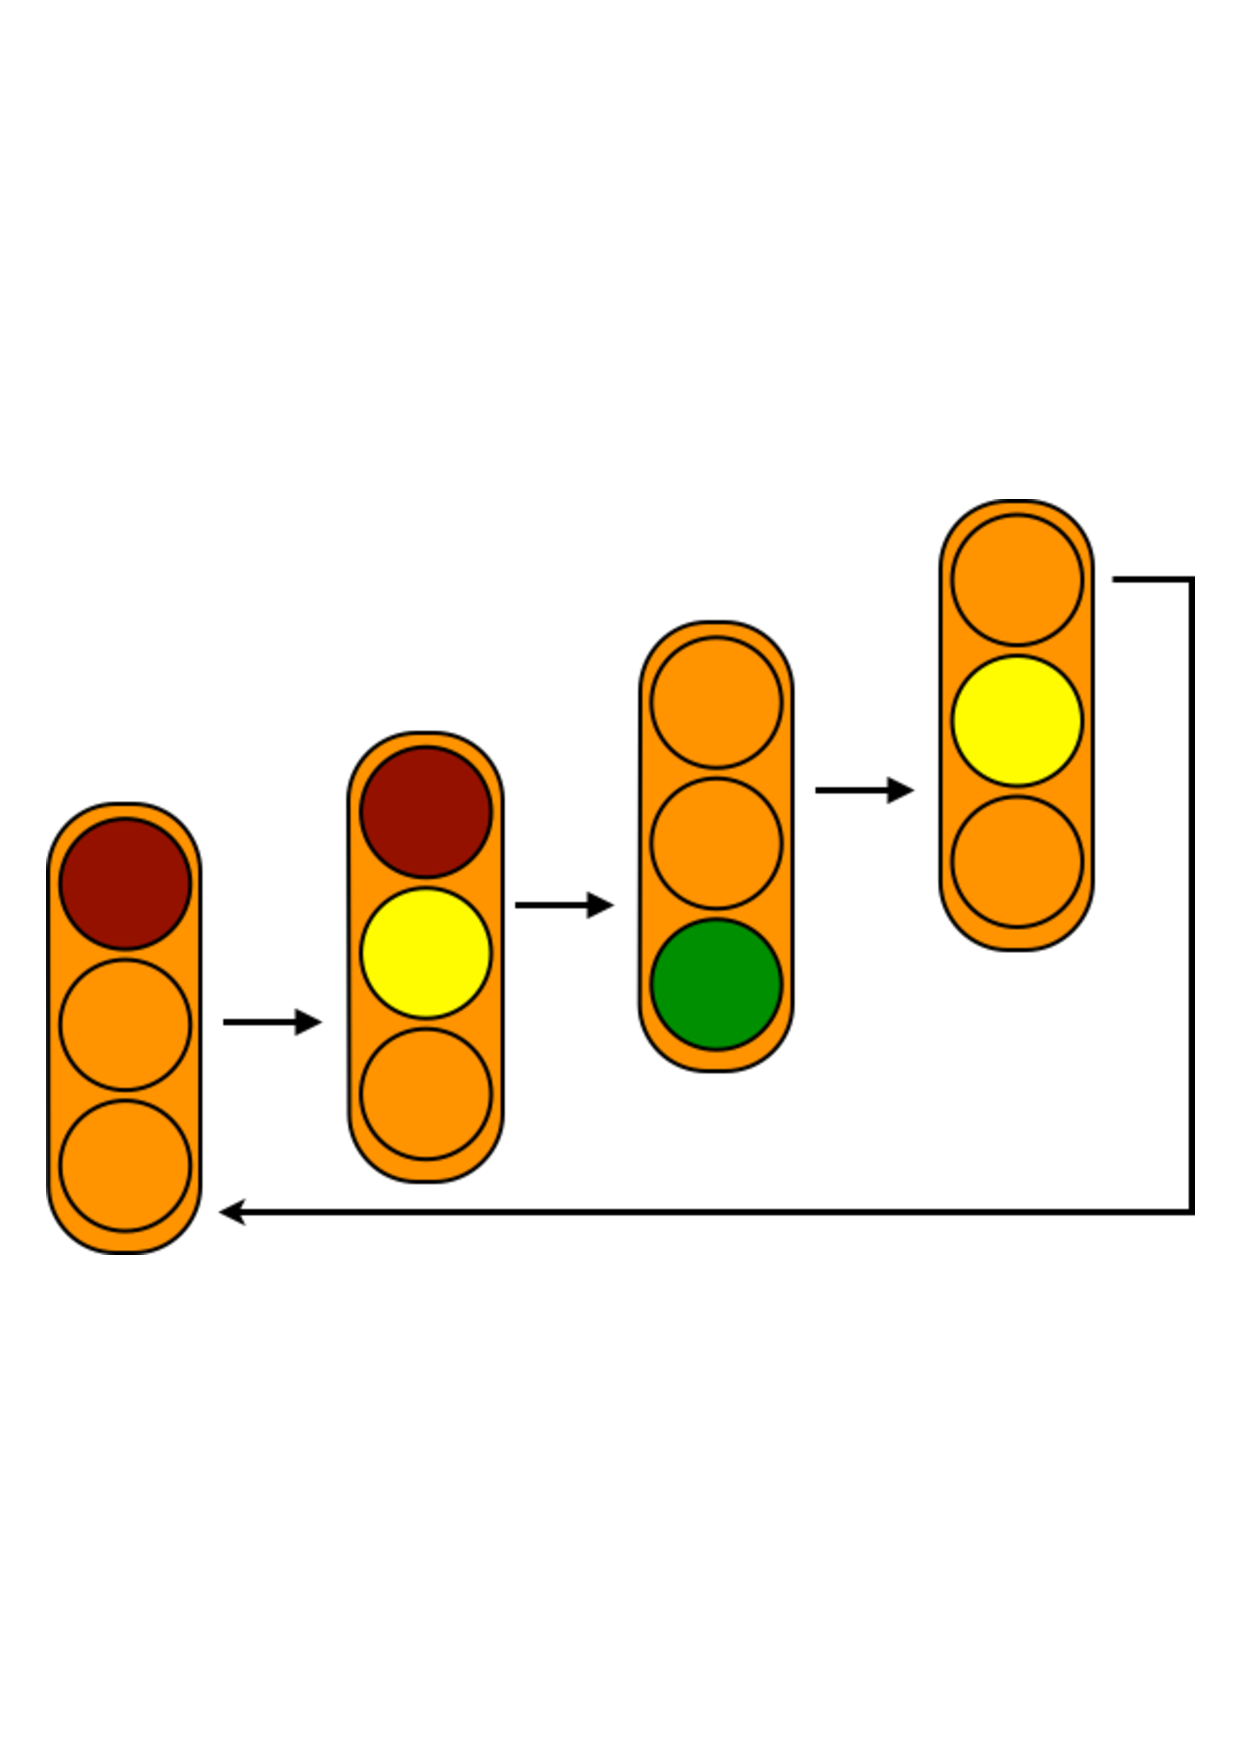
\includegraphics{images/full-light.pdf}}
\end{center}
\end{exc}

\section{Defining specifications as propositions}
\label{sec:spec}

Consider the following property which we might want to check
for our system:
%
\begin{quote}
\emph{If we are in a valid state and change state, then our new state
  is also valid.}
\end{quote}
%
We can abstract the notion of a valid state with the following
meta-level operation (you can think of this as a syntax function mapping from the
two propositions to a proposition):
%
\begin{equation*}
\textsf{valid-state}(r, g) = (r \wedge \neg g) \vee (\neg r \wedge g)
\end{equation*}
%
From this, we can then capture our specification as the proposition:
%
\begin{equation*}
  \textit{specification} = \textsf{valid-state}(\atomr, \atomg)
  \rightarrow \textsf{valid-state}(\atomrp, \atomgp)
\end{equation*}
%
\ie{}, a valid state now implies a valid state in the next time step.
To verify that our system (based on its model) satisfies this
property, we then need to prove that the following is true:
%
\begin{align*}
 & \textit{model} \rightarrow \textit{specification} \\
  \equiv \; &
((\atomr{} \wedge \neg\atomg{} \; \rightarrow \; \neg\atomr{}' \wedge
\atomg{}')
\wedge
(\neg\atomr{} \wedge \atomg{} \; \rightarrow \; \atomr{}' \wedge
  \neg\atomg{}'))
  \rightarrow
   (\textsf{valid-state}(\atomr, \atomg)
           \rightarrow \textsf{valid-state}(\atomrp, \atomgp)) \\
  \equiv \; &
((\atomr{} \wedge \neg\atomg{} \; \rightarrow \; \neg\atomr{}' \wedge
\atomg{}')
\wedge
(\neg\atomr{} \wedge \atomg{} \; \rightarrow \; \atomr{}' \wedge
  \neg\atomg{}'))
              \rightarrow
              (((\atomr \wedge \neg \atomg) \vee (\neg \atomr \wedge \atomg))
              \rightarrow ((\atomrp \wedge \neg \atomgp) \vee (\neg \atomrp \wedge \atomgp)))
\end{align*}
%
This is quite a big proposition so we might not want to prove it by
hand. Instead, in the next part of the course we are going to use an
algorithmic technique for proving that this holds (Part C,
specifically \textbf{Example 5} in the notes). We will later see that
this does indeed hold, and thus the system (as described by the model)
satisfies our specification.


\section{When is a model a good model?}
\label{subsec:whenisamodelgood}

\begin{quote}
\emph{All models are wrong but some are useful} (Box, 1978)
\end{quote}

\noindent
Indeed, a model is necessarily ``wrong'' in the sense that a model
abstracts some of the details of a real system; we are not
capturing every aspect of the system, such as: how are the transitions
triggered? or, what happens if a car crashes into the traffic light? Some
models, though eliding details, are useful in the sense that we
can detect when the system does not behave according to our
specification or we can verify that it always behaves according to our
specification. Just enough detail is needed in the model to capture what
we want to prove.

Our running example has the model:
\begin{equation*}
\mathit{model} =
(\atomr{} \wedge \neg\atomg{} \; \rightarrow \; \neg\atomr{}' \wedge
\atomg{}')
\wedge
(\neg\atomr{} \wedge \atomg{} \; \rightarrow \; \atomr{}' \wedge \neg\atomg{}')
\end{equation*}
%
We might add to this model the explicit exclusion of invalid
states. Let's define the condition of the invalid states via the meta-level function:
%
\begin{equation*}
\textsf{invalid-state}(r, g) = (\neg r \wedge \neg g) \vee (r \wedge g)
\end{equation*}
%
Then we could define an alternate model as:
%
\begin{equation*}
\mathit{model2} = \mathit{model} \wedge \neg \textsf{invalid-state}(\atomr, \atomg)
\end{equation*}
%
Thus, the new model adds to the old model that the current state is not
invalid.

In the case of the proving our specification from
Section~\ref{sec:spec} (that valid states transition to valid states)
we do not need this additional detail in the model. But we might want
to have this more restrictive model if we want to prove, for example,
that we can never be in an invalid state, regardless of what state we
started from. This can be captured by the new specification:
%
\begin{equation*}
\mathit{specification2} = \textsf{invalid-state}(\atomr, \atomg)
\vee \textsf{invalid-state}(\atomr', \atomg')
\end{equation*}
%
and proving that the following proposition is valid:
$$
\mathit{model2} \rightarrow
\neg \mathit{specification2}
$$
Note we are using a negative property
here: we show that the new model (\textit{model2}) implies that the bad behaviour is not possible.
For the old model (\textit{model}), a similar proposition capturing the same idea is valid:
$$
\mathit{model} \rightarrow \neg \mathit{specification2}
$$
However, the following proposition is also valid!!!
$$
\mathit{model} \rightarrow \mathit{specification2}
$$
Why? If the right-hand side of the implication is true (we have an
invalid state) the left-hand side is still true (the premise of each
transition implication is false, therefore the implications are
trivially true); the original model never excludes invalid states on
their own, only as the result of a transition from a valid
state. Thus, the original model was not a good model for checking the
$\mathit{specification2}$ property, but it was sufficient for
$\mathit{specification}$.

Creating a rich enough model is up to you, and requires some care and
thought about the domain and what properties are of interest.
